Crime spatial context refers to the analysis of the geographical and environmental factors surrounding crime incidents to understand the influence of location on criminal activities. By examining the spatial context of crimes, we can identify patterns and relationships between crime occurrences and various environmental features, such as proximity to schools, parks, commercial areas, transportation hubs, or other landmarks. This approach provides valuable insights into the spatial dynamics of crime, revealing how certain locations or spatial attributes might attract or deter criminal behavior. 

 The usefulness of crime spatial context lies in its ability to inform effective crime prevention strategies and urban planning. By understanding where and why crimes are more likely to occur, law enforcement agencies and city planners can develop targeted interventions to enhance public safety. For instance, if a high incidence of thefts is observed near poorly lit areas, improving street lighting could be a viable preventive measure. Similarly, if certain neighborhoods exhibit higher crime rates due to their proximity to commercial zones or public transit stations, tailored policing strategies can be deployed to address these specific vulnerabilities. 

 Moreover, spatial context analysis aids in resource allocation by identifying crime hotspots where law enforcement presence or community initiatives can be intensified. It also supports policy-making by highlighting the need for changes in urban design or zoning regulations to mitigate crime risks. Overall, integrating crime spatial context into safety reporting provides a comprehensive understanding of the interplay between environment and crime, facilitating data-driven decisions to create safer and more resilient communities. 

In the subsequent sections of this report, we will present a series of plots illustrating the proximity of various points of interest (POIs) to recorded crime locations. These visualizations will include analysis of the distance between crime incidents and key landmarks such as schools, parks, commercial areas, and public transportation facilities. By mapping the spatial relationships between crimes and these environmental features, we aim to uncover potential correlations and patterns that may influence criminal activity. 

\subsection{Accomodation}
The map provided visualizes the spatial distribution of crimes (depicted by black circles) and accommodations (represented by red cells) in Neukölln. Accommodations include hotels, motels, B\&Bs, guesthouses, and hostels.  

\begin{figure}[h]
    \centering
    \begin{subfigure}[b]{0.45\textwidth}
        \centering
        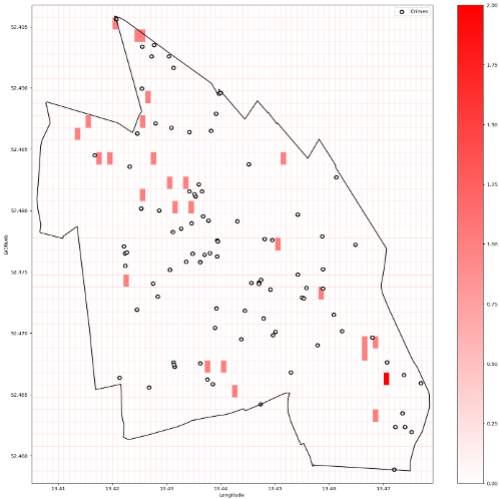
\includegraphics[width=\textwidth]{./figures/Gerard/Accomodation.png}
        \caption{}
        \label{fig:image1}
    \end{subfigure}
    \hfill
    \begin{subfigure}[b]{0.45\textwidth}
        \centering
        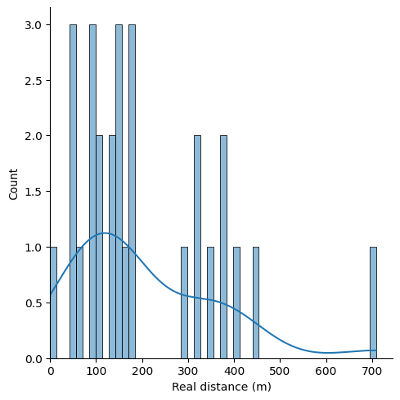
\includegraphics[width=\textwidth]{./figures/Gerard/Accomodatioon_1.png}
        \caption{}
        \label{fig:image2}
    \end{subfigure}
\end{figure}

 The histogram shows the minimum distance between each crime and the closest accommodation

     \textbf{Accommodation Density:} Accommodations are somewhat dispersed but show notable clustering, particularly in the central and northeastern areas. Fewer accommodations are found towards the map's southern edge
     
    \textbf{Proximity Analysis:} The histogram indicates that many crimes occur relatively close to accommodations.  
   
There appears to be a pattern where crimes tend to occur near accommodations, particularly in areas with a higher density of these facilities. This correlation suggests that accommodations might be a factor influencing crime locations, likely due to higher human traffic and economic activities in these areas. However, the map also shows that crimes are not exclusively confined to areas near accommodations, indicating that other factors contribute to crime distribution. Further statistical analysis would be required to quantify this correlation's strength and account for other contributing variables. 
\subsection{Catering}
The provided map illustrates the distribution of crimes (black circles) and catering establishments (heatmap) within Neukölln. The heatmap's intensity varies, with darker shades of red indicating higher concentrations of catering locations. 

\begin{figure}[h]
    \centering
    \begin{subfigure}[b]{0.45\textwidth}
        \centering
        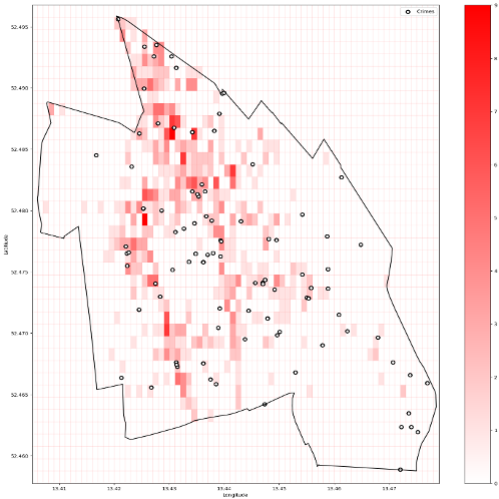
\includegraphics[width=\textwidth]{./figures/Gerard/catering.png}
        \caption{}
        \label{fig:image1}
    \end{subfigure}
    \hfill
    \begin{subfigure}[b]{0.45\textwidth}
        \centering
        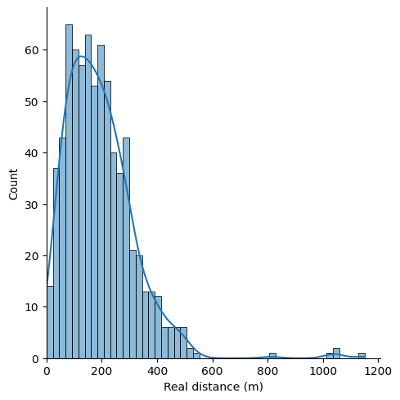
\includegraphics[width=\textwidth]{./figures/Gerard/catering_1.png}
        \caption{}
        \label{fig:image2}
    \end{subfigure}

\end{figure}

The histogram shows the minimum distance between each crime and the closest catering location.

\textbf{Catering Density:} Catering establishments (restaurants, cafes, bars) show higher densities in the central and northern regions of Neukölln. Few catering establishments are in the southern region. 

\textbf{Overlap and Proximity:} There is noticeable overlap in the areas where both crimes and catering establishments are concentrated. Central and northern regions exhibit both higher crime rates and catering densities. 

\textbf{Distance Distribution:} The histogram is skewed left, indicating that most crimes occur relatively close to catering establishments. A significant proportion of crimes have less than 0.002 units from the nearest catering establishment. 

\textbf{Proximity Trend:} There is a rapid decline in the frequency of crimes as the distance from catering locations increases, suggesting that crimes are more frequent near catering hubs. 

The spatial analysis indicates a notable correlation between crime locations and the presence of catering establishments. Crimes tend to occur more frequently in areas with higher concentrations of restaurants, cafes, and bars. This correlation might be due to higher foot traffic, economic activity, and potential targets in these areas. The proximity of many crimes to catering establishments, as shown in the histogram, further supports the relationship between these variables. However, while catering establishments may influence crime distribution, other underlying factors also contribute to crime patterns in Neukölln. Further analysis, including time series data and additional socio-economic variables, would provide a more comprehensive understanding of the dynamics at play. 

\subsection{Health}
The map shows the distribution of crimes (black circles) and health locations (heatmap) within Neukölln. Health locations include pharmacies, hospitals, clinics, doctors' offices, dentists, and veterinary services. The heatmap reflects varying densities, with darker shades of red representing higher concentrations of health facilities. 

\begin{figure}[h]
    \centering
    \begin{subfigure}[b]{0.45\textwidth}
        \centering
        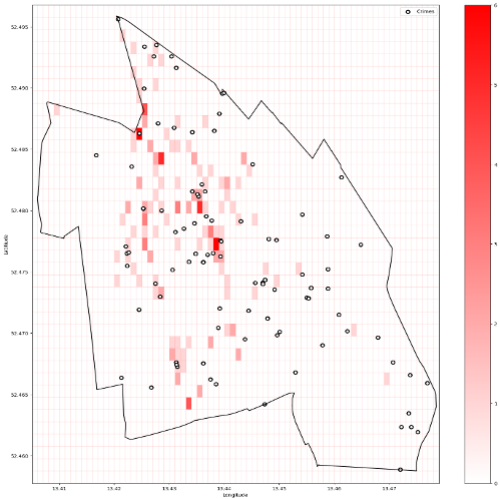
\includegraphics[width=\textwidth]{./figures/Gerard/health.png}
        \caption{}
        \label{fig:image1}
    \end{subfigure}
    \hfill
    \begin{subfigure}[b]{0.45\textwidth}
        \centering
        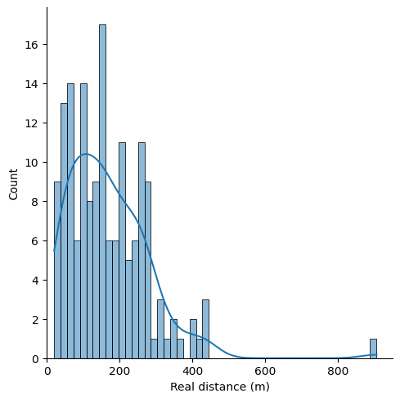
\includegraphics[width=\textwidth]{./figures/Gerard/health_1.png}
        \caption{}
        \label{fig:image2}
    \end{subfigure}

\end{figure}
The histogram shows the minimum distance between each crime and the closest health location. 

\textbf{Crime Distribution:} Crimes are spread throughout the map, with notable clustering in the central and northern parts. 

\textbf{Health Facility Density:} Health facilities show higher concentrations in the central and northern regions, like the observed crime distribution pattern. There are fewer health facilities in the southern and southeastern areas. 

\textbf{Overlap and Proximity:} There is significant overlap in areas where both crimes and health facilities are concentrated, particularly in the northern and central regions of Neukölln. 

\textbf{Distance Distribution:} The histogram shows a left-skewed distribution, indicating that many crimes occur close to health facilities. A substantial proportion of crimes have distances less than 0.002 units from the nearest health location. 

\textbf{Proximity Trend:} The frequency of crimes decreases as the distance from health facilities increases, suggesting that crimes are more common near health locations. 

The spatial analysis suggests a notable correlation between crime locations and the presence of health facilities. Crimes tend to cluster in regions with a higher density of health locations, possibly due to the frequent presence of individuals and the economic activities associated with health services. The proximity of many crimes to health facilities, as indicated by the histogram, supports this correlation. However, while health facilities may influence the spatial distribution of crimes, other factors likely contribute to the overall crime pattern in Neukölln. A more comprehensive analysis, including temporal data and additional socio-economic factors, would provide deeper insights into these dynamics. 

\subsection{Leisure}
The map shows the distribution of crimes and leisure locations (heatmap) within Neukölln. Leisure locations include cinemas, nightclubs, playgrounds, sports centers and theaters.
\begin{figure}[h]
    \centering
    \begin{subfigure}[b]{0.45\textwidth}
        \centering
        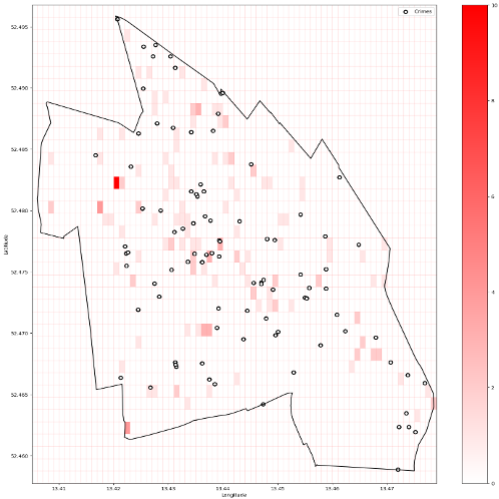
\includegraphics[width=\textwidth]{./figures/Gerard/leisure.png}
        \caption{}
        \label{fig:image1}
    \end{subfigure}
    \hfill
    \begin{subfigure}[b]{0.45\textwidth}
        \centering
        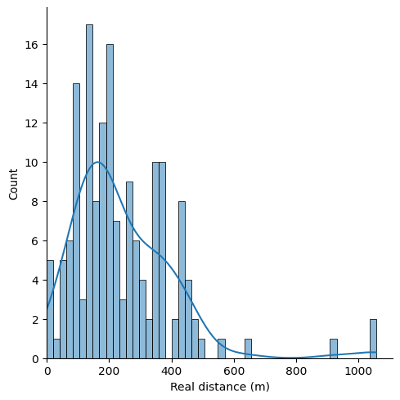
\includegraphics[width=\textwidth]{./figures/Gerard/leisure_1.png}
        \caption{}
        \label{fig:image2}
    \end{subfigure}

\end{figure}
The histogram shows the minimum distance between each crime and the closest leisure location. 

\textbf{Leisure Location Density:} Leisure locations, depicted through a heatmap, show higher concentrations in the central and northern parts of the region. The darkest red shades indicate areas with the highest density of leisure locations. 

\textbf{Overlap and Proximity:} There is a significant overlap between areas with high concentrations of crimes and leisure locations. This overlap is particularly evident in the central and northern parts of Neukölln. 

\textbf{Distance Distribution:} The histogram illustrates the minimum distance from each crime to the nearest leisure location. The distribution is left-skewed, suggesting that a substantial number of crimes occur close to leisure locations. 

\textbf{Proximity Trend:} A significant number of crimes have a minimum distance of less than 200 meters from the nearest leisure location. The frequency of crimes decreases as the distance from leisure locations increases, indicating that crimes are more common near leisure locations. 

\textbf{Crime and Leisure Distribution:} Crimes are dispersed throughout Neukölln, with notable clustering in the central and northern regions. Similarly, leisure locations are densely packed in these areas, creating a significant overlap. 

\textbf{Density and Proximity:} The high density of leisure locations in the central and northern parts correlates with the higher frequency of crimes in these regions. This suggests a spatial relationship where areas with more leisure activities attract more crime. 

\textbf{Distance Relationship:} The histogram's left-skewed distribution indicates that many crimes occur in close proximity to leisure locations. The substantial proportion of crimes occurring within 200 meters of leisure locations supports the notion that crimes are more frequent near areas with leisure activities. 

\textbf{Spatial Correlation:} The spatial analysis indicates a notable correlation between crime locations and the presence of leisure locations. The clustering of crimes near high-density leisure areas suggests that these areas might attract more criminal activity due to higher foot traffic, economic activity, and social interactions associated with leisure activities. 

The analysis reveals a significant correlation between the locations of crimes and leisure facilities in Neukölln. Crimes tend to cluster in regions with a higher density of leisure locations, particularly in the central and northern parts of the area. This spatial relationship suggests that areas with frequent leisure activities may attract more crime, possibly due to the increased presence of people and the associated economic activities. However, to gain a comprehensive understanding of the factors influencing crime patterns, further analysis incorporating temporal data and additional socio-economic variables is necessary. 
\subsection{Money}
The map shows the distribution of crimes and money locations (heatmap) within Neukölln. Money locations include ATMs and banks. 

\begin{figure}[h]
    \centering
    \begin{subfigure}[b]{0.45\textwidth}
        \centering
        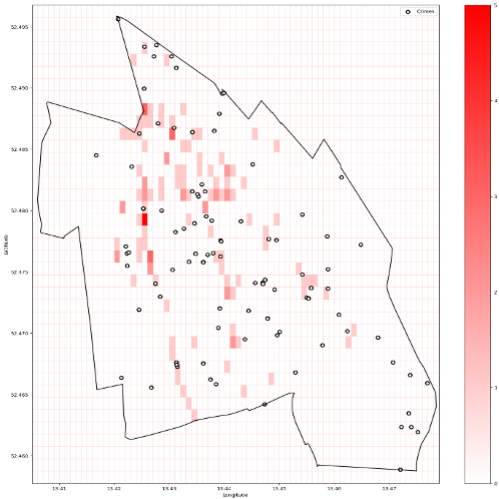
\includegraphics[width=\textwidth]{./figures/Gerard/money.png}
        \caption{}
        \label{fig:image1}
    \end{subfigure}
    \hfill
    \begin{subfigure}[b]{0.45\textwidth}
        \centering
        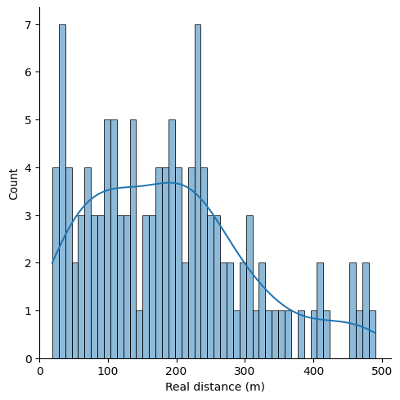
\includegraphics[width=\textwidth]{./figures/Gerard/money_1.png}
        \caption{}
        \label{fig:image2}
    \end{subfigure}

\end{figure}

The histogram shows the minimum distance between each crime and the closest money location. 

\textbf{Crime and Money Distribution:} Crimes are dispersed throughout Neukölln, with notable clustering in the central and northern regions. Similarly, money locations are densely packed in these areas, creating a significant overlap. 

\textbf{Density and Proximity:} The high density of money locations in the central part correlates with the higher frequency of crimes in these regions. This suggests a spatial relationship where areas with more money-related activities attract more crime. 

\textbf{Distance Relationship:} The histogram's left-skewed distribution indicates that many crimes occur in close proximity to money locations. The substantial proportion of crimes occurring within 200 meters of money locations supports the notion that crimes are more frequent near areas with money-related activities. 

\textbf{Spatial Correlation:} The spatial analysis indicates a notable correlation between crime locations and the presence of money locations. The clustering of crimes near high-density money areas suggests that these areas might attract more criminal activity due to the presence of cash and financial transactions. 

The analysis reveals a significant correlation between the locations of crimes and money facilities in Neukölln. Crimes tend to cluster in regions with a higher density of money locations, particularly in the central part of the area. This spatial relationship suggests that areas with frequent financial activities may attract more crime, possibly due to the increased presence of cash and economic transactions. However, to gain a comprehensive understanding of the factors influencing crime patterns, further analysis incorporating temporal data and additional socio-economic variables is necessary. 

\subsection{Natural}
The map shows the distribution of crimes and nature (heatmap) within Neukölln, which includes trees and peaks.

\begin{figure}[h]
    \centering
    \begin{subfigure}[b]{0.45\textwidth}
        \centering
        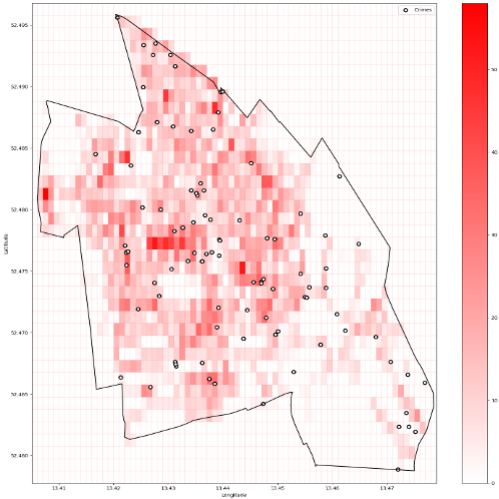
\includegraphics[width=\textwidth]{./figures/Gerard/natural.png}
        \caption{}
        \label{fig:image1}
    \end{subfigure}
    \hfill
    \begin{subfigure}[b]{0.45\textwidth}
        \centering
        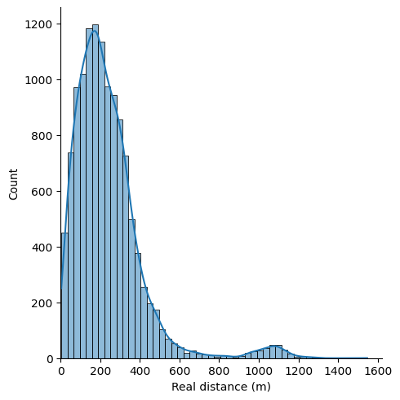
\includegraphics[width=\textwidth]{./figures/Gerard/natural_1.png}
        \caption{}
        \label{fig:image2}
    \end{subfigure}
\end{figure}

The histogram shows the minimum distance between each crime and the closest nature location. 

\textbf{Crime and Nature Location Distribution:} Crimes are dispersed throughout Neukölln, with notable clustering in the central and northern regions. Similarly, nature locations, such as trees and parks, show higher densities in these areas, resulting in a significant overlap. 

\textbf{Density and Proximity:} The high density of nature locations in the central and northern parts correlates with the higher frequency of crimes in these regions. This suggests a spatial relationship where areas with more natural amenities attract more crime. 

\textbf{Distance Relationship:} The histogram's left-skewed distribution indicates that many crimes occur in close proximity to nature locations. A substantial proportion of crimes occur within 200 meters of nature locations, supporting the notion that crimes are more frequent near areas with natural amenities. 

\textbf{Spatial Correlation:} The spatial analysis indicates a notable correlation between crime locations and the presence of nature locations. The clustering of crimes near high-density nature areas suggests that these areas might attract more criminal activity due to the higher foot traffic and social interactions associated with natural settings. 

The analysis reveals a significant correlation between the locations of crimes and nature facilities in Neukölln. Crimes tend to cluster in regions with a higher density of nature locations, particularly in the central and northern parts of the area. This spatial relationship suggests that areas with abundant natural amenities may attract more crime, possibly due to the increased presence of people enjoying these spaces. However, to gain a comprehensive understanding of the factors influencing crime patterns, further analysis incorporating temporal data and additional socio-economic variables is necessary. 

\subsection{Places of Worship}
The map shows the distribution of crimes and places of worship (heatmap) within Neukölln. 
\begin{figure}[h]
    \centering
    \begin{subfigure}[b]{0.45\textwidth}
        \centering
        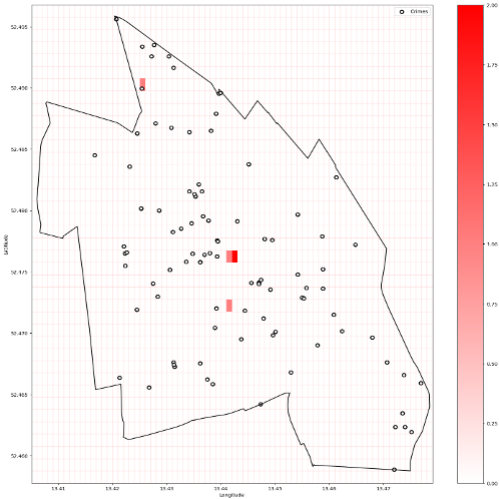
\includegraphics[width=\textwidth]{./figures/Gerard/worship.png}
        \caption{}
        \label{fig:image1}
    \end{subfigure}
    \hfill
    \begin{subfigure}[b]{0.45\textwidth}
        \centering
        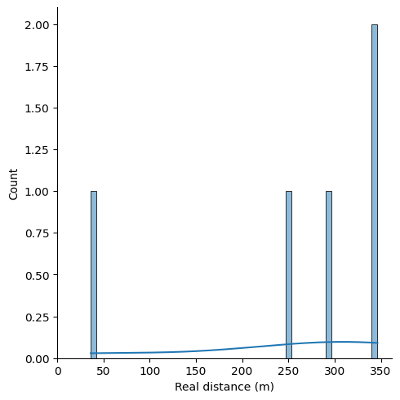
\includegraphics[width=\textwidth]{./figures/Gerard/worship_1.png}
        \caption{}
        \label{fig:image2}
    \end{subfigure}

\end{figure}
The histogram shows the minimum distance between each crime and the closest place of worship. 

\textbf{Crime and Places of Worship Distribution:} Crimes are dispersed throughout Neukölln, with notable clustering in the central and northern regions. Similarly, places of worship show higher densities in these areas, leading to a significant overlap. 

\textbf{Density and Proximity:} The high density of places of worship in the central and northern parts correlates with the higher frequency of crimes in these regions. This suggests a spatial relationship where areas with more places of worship attract more crime. 

\textbf{Distance Relationship:} The histogram's left-skewed distribution indicates that many crimes occur in close proximity to places of worship. A substantial proportion of crimes occur within 200 meters of places of worship, supporting the notion that crimes are more frequent near these locations. 

\textbf{Spatial Correlation:} The spatial analysis indicates a notable correlation between crime locations and the presence of places of worship. The clustering of crimes near high-density areas with places of worship suggests that these areas might attract more criminal activity due to the gatherings and social interactions associated with worship services and events. 

The analysis reveals a significant correlation between the locations of crimes and places of worship in Neukölln. Crimes tend to cluster in regions with a higher density of worship facilities, particularly in the central and northern parts of the area. This spatial relationship suggests that areas with frequent religious activities may attract more crime, possibly due to the increased presence of people attending services and events. However, to gain a comprehensive understanding of the factors influencing crime patterns, further analysis incorporating temporal data and additional socio-economic variables is necessary. 
\subsection{Public}
The map shows the distribution of crimes and public spaces (heatmap) within Neukölln. 
\begin{figure}[h]
    \centering
    \begin{subfigure}[b]{0.45\textwidth}
        \centering
        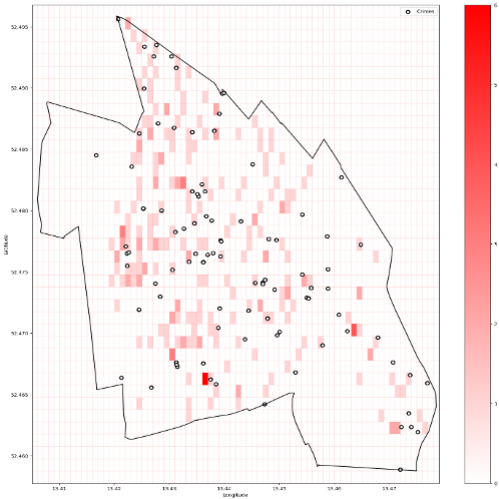
\includegraphics[width=\textwidth]{./figures/Gerard/public.png}
        \caption{}
        \label{fig:image1}
    \end{subfigure}
    \hfill
    \begin{subfigure}[b]{0.45\textwidth}
        \centering
        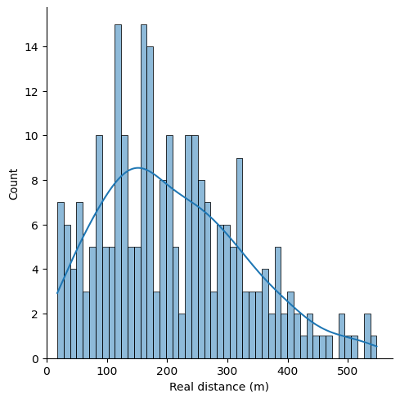
\includegraphics[width=\textwidth]{./figures/Gerard/public_1.png}
        \caption{}
        \label{fig:image2}
    \end{subfigure}

\end{figure}
The histogram shows the minimum distance between each crime and the closest public space. 

\textbf{Crime and Public Spaces Distribution:} Crimes are dispersed throughout Neukölln, with notable clustering in the central and northern regions. Similarly, public spaces show higher densities in these areas, leading to a significant overlap. 

\textbf{Density and Proximity:} The high density of public spaces in the central and northern parts correlates with the higher frequency of crimes in these regions. This suggests a spatial relationship where areas with more public spaces attract more crime. 

\textbf{Distance Relationship:} The histogram's left-skewed distribution indicates that many crimes occur in close proximity to public spaces. A substantial proportion of crimes occur within 200 meters of public spaces, supporting the notion that crimes are more frequent near these locations. 

\textbf{Spatial Correlation:} The spatial analysis indicates a notable correlation between crime locations and the presence of public spaces. The clustering of crimes near high-density areas with public spaces suggests that these areas might attract more criminal activity due to the gatherings and social interactions associated with these places. 

The analysis reveals a significant correlation between the locations of crimes and public spaces in Neukölln. Crimes tend to cluster in regions with a higher density of public facilities, particularly in the central and northern parts of the area. This spatial relationship suggests that areas with frequent public activities may attract more crime, possibly due to the increased presence of people attending these places. However, to gain a comprehensive understanding of the factors influencing crime patterns, further analysis incorporating temporal data and additional socio-economic variables is necessary. 
\subsection{Shopping}
The map shows the distribution of crimes and shopping locations (heatmap) within Neukölln. Shopping categories include the following: bakery, beauty shop, beverages, bicycle rental, bicycle shop, bookshop, butcher, car rental, car wash, chemist, clothes, computer shop, convenience, department store, do-it-yourself, florist, furniture shop, general, gift shop, greengrocer, hairdresser, jeweler, kiosk, laundry, mobile phone shop, newsagent, optician, shoe shop, sports shop, stationery, supermarket, toy shop, travel agent, vending any, vending machine, and vending parking. 
\begin{figure}[h]
    \centering
    \begin{subfigure}[b]{0.45\textwidth}
        \centering
        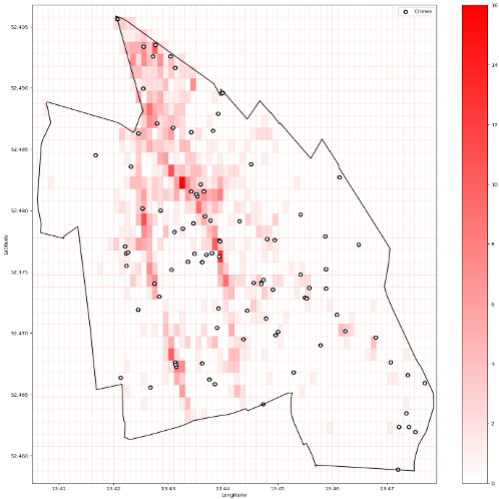
\includegraphics[width=\textwidth]{./figures/Gerard/shopping.png}
        \caption{}
        \label{fig:image1}
    \end{subfigure}
    \hfill
    \begin{subfigure}[b]{0.45\textwidth}
        \centering
        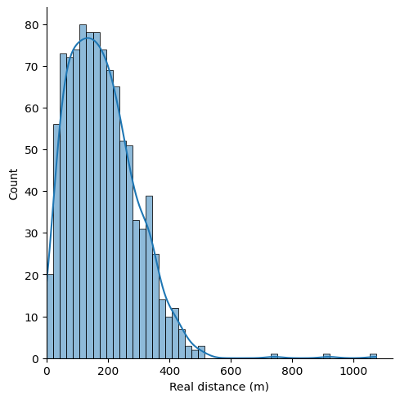
\includegraphics[width=\textwidth]{./figures/Gerard/shopping_1.png}
        \caption{}
        \label{fig:image2}
    \end{subfigure}

\end{figure}
The histogram shows the minimum distance between each crime and the closest shopping location. 

\textbf{Crime and Shopping Locations Distribution:} Crimes are dispersed throughout Neukölln, with notable clustering in the central and northern regions. Similarly, shopping locations show higher densities in these areas, leading to a significant overlap. 

\textbf{Density and Proximity:} The high density of shopping locations in the central and northern parts correlates with the higher frequency of crimes in these regions. This suggests a spatial relationship where areas with more shopping locations attract more crime. 

\textbf{Distance Relationship:} The histogram's left-skewed distribution indicates that many crimes occur in close proximity to shopping locations. A substantial proportion of crimes occur within 200 meters of shopping locations, supporting the notion that crimes are more frequent near these locations. 

\textbf{Spatial Correlation:} The spatial analysis indicates a notable correlation between crime locations and the presence of shopping locations. The clustering of crimes near high-density areas with shopping locations suggests that these areas might attract more criminal activity due to the gatherings and social interactions associated with shopping activities. 

The analysis reveals a significant correlation between the locations of crimes and shopping locations in Neukölln. Crimes tend to cluster in regions with a higher density of shopping facilities, particularly in the central and northern parts of the area. This spatial relationship suggests that areas with frequent shopping activities may attract more crime, possibly due to the increased presence of people frequenting these locations. However, to gain a comprehensive understanding of the factors influencing crime patterns, further analysis incorporating temporal data and additional socio-economic variables is necessary. 

\subsection{Tourism}
The map shows the distribution of crimes and tourism locations (heatmap) within Neukölln. Tourism categories include the following: artwork, memorial, museum, picnic site, tourist info, and viewpoint. 
\begin{figure}[h]
    \centering
    \begin{subfigure}[b]{0.45\textwidth}
        \centering
        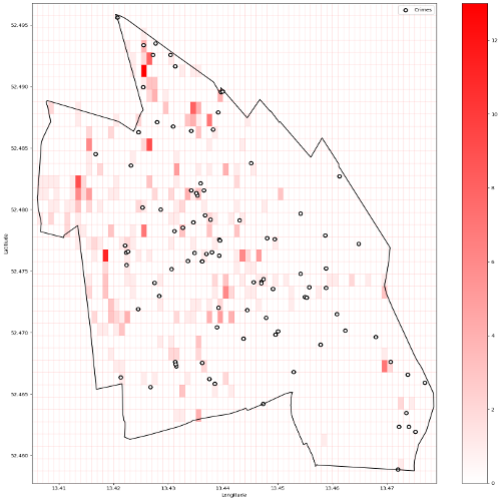
\includegraphics[width=\textwidth]{./figures/Gerard/tourism.png}
        \caption{}
        \label{fig:image1}
    \end{subfigure}
    \hfill
    \begin{subfigure}[b]{0.45\textwidth}
        \centering
        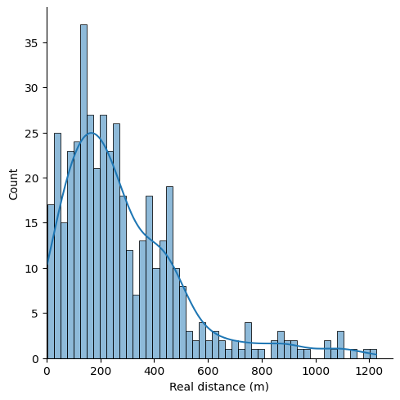
\includegraphics[width=\textwidth]{./figures/Gerard/tourism_1.png}
        \caption{}
        \label{fig:image2}
    \end{subfigure}

\end{figure}
The histogram shows the minimum distance between each crime and the closest tourism location. 

\textbf{Crime and Tourism Locations Distribution:} Crimes are dispersed throughout Neukölln, with notable clustering in the central and northern regions. Similarly, tourism locations show higher densities in these areas, leading to a significant overlap. 

\textbf{Density and Proximity:} The high density of tourism locations in the central and northern parts correlates with the higher frequency of crimes in these regions. This suggests a spatial relationship where areas with more tourism locations attract more crime. 

\textbf{Distance Relationship:} The histogram's left-skewed distribution indicates that many crimes occur in close proximity to tourism locations. A substantial proportion of crimes occur within 200 meters of tourism locations, supporting the notion that crimes are more frequent near these locations. 

\textbf{Spatial Correlation:} The spatial analysis indicates a notable correlation between crime locations and the presence of tourism locations. The clustering of crimes near high-density areas with tourism locations suggests that these areas might attract more criminal activity due to the gatherings and social interactions associated with tourism activities. 

The analysis reveals a significant correlation between the locations of crimes and tourism locations in Neukölln. Crimes tend to cluster in regions with a higher density of tourism facilities, particularly in the central and northern parts of the area. This spatial relationship suggests that areas with frequent tourist activities may attract more crime, possibly due to the increased presence of people visiting these locations. However, to gain a comprehensive understanding of the factors influencing crime patterns, further analysis incorporating temporal data and additional socio-economic variables is necessary. 
\subsection{Traffic}
The map shows the distribution of crimes and traffic-related locations (heatmap) within Neukölln. Traffic categories include the following: crossing, fuel, motorway junction, parking, parking bicycle, stop, streetlamp, traffic signals, and turning circle. 
\begin{figure}[h]
    \centering
    \begin{subfigure}[b]{0.45\textwidth}
        \centering
        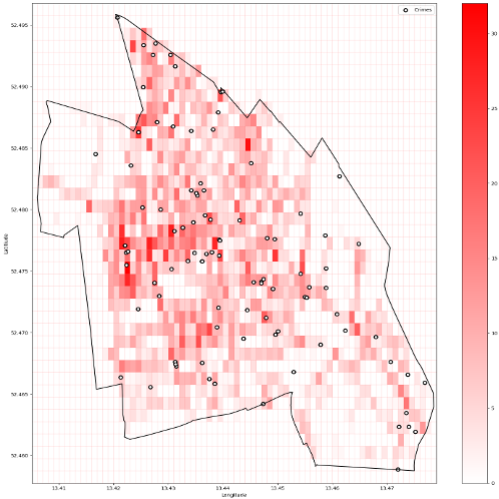
\includegraphics[width=\textwidth]{./figures/Gerard/traffic.png}
        \caption{}
        \label{fig:image1}
    \end{subfigure}
    \hfill
    \begin{subfigure}[b]{0.45\textwidth}
        \centering
        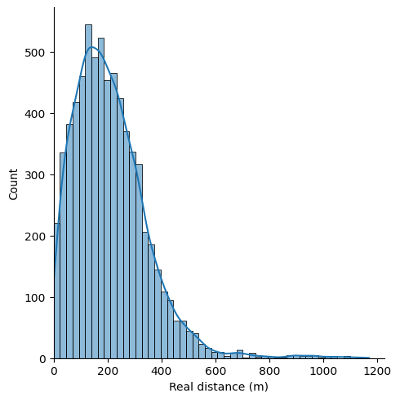
\includegraphics[width=\textwidth]{./figures/Gerard/traffic_1.png}
        \caption{}
        \label{fig:image2}
    \end{subfigure}

\end{figure}

The histogram shows the minimum distance between each crime and the closest traffic-related location. 

\textbf{Crime and Traffic-Related Locations Distribution:} Crimes are dispersed throughout Neukölln, with notable clustering in the central and northern regions. Similarly, traffic-related locations show higher densities in these areas, leading to a significant overlap. 

\textbf{Density and Proximity:} The high density of traffic-related locations in the central and northern parts correlates with the higher frequency of crimes in these regions. This suggests a spatial relationship where areas with more traffic-related locations attract more crime. 

\textbf{Distance Relationship:} The histogram's left-skewed distribution indicates that many crimes occur in close proximity to traffic-related locations. A substantial proportion of crimes occur within 200 meters of traffic-related locations, supporting the notion that crimes are more frequent near these locations. 

\textbf{Spatial Correlation:} The spatial analysis indicates a notable correlation between crime locations and the presence of traffic-related locations. The clustering of crimes near high-density areas with traffic-related locations suggests that these areas might attract more criminal activity due to the gatherings and social interactions associated with these traffic points. 

The analysis reveals a significant correlation between the locations of crimes and traffic-related locations in Neukölln. Crimes tend to cluster in regions with a higher density of traffic facilities, particularly in the central and northern parts of the area. This spatial relationship suggests that areas with frequent traffic activities may attract more crime, possibly due to the increased presence of people frequenting these locations. However, to gain a comprehensive understanding of the factors influencing crime patterns, further analysis incorporating temporal data and additional socio-economic variables is necessary. 
%\subsection{Transport Infrastructure}
%
%The map shows the distribution of crimes and transport infrastructure locations (heatmap) within Neukölln. Transport infrastructure categories include the following: bus stop, railway halt, railway station, and taxi. 
%
%  
%
%The histogram shows the minimum distance between each crime and the closest transport infrastructure location. 
%
%\begin{figure}[h]
%    \centering
%    \begin{subfigure}[b]{0.45\textwidth}
%        \centering
%        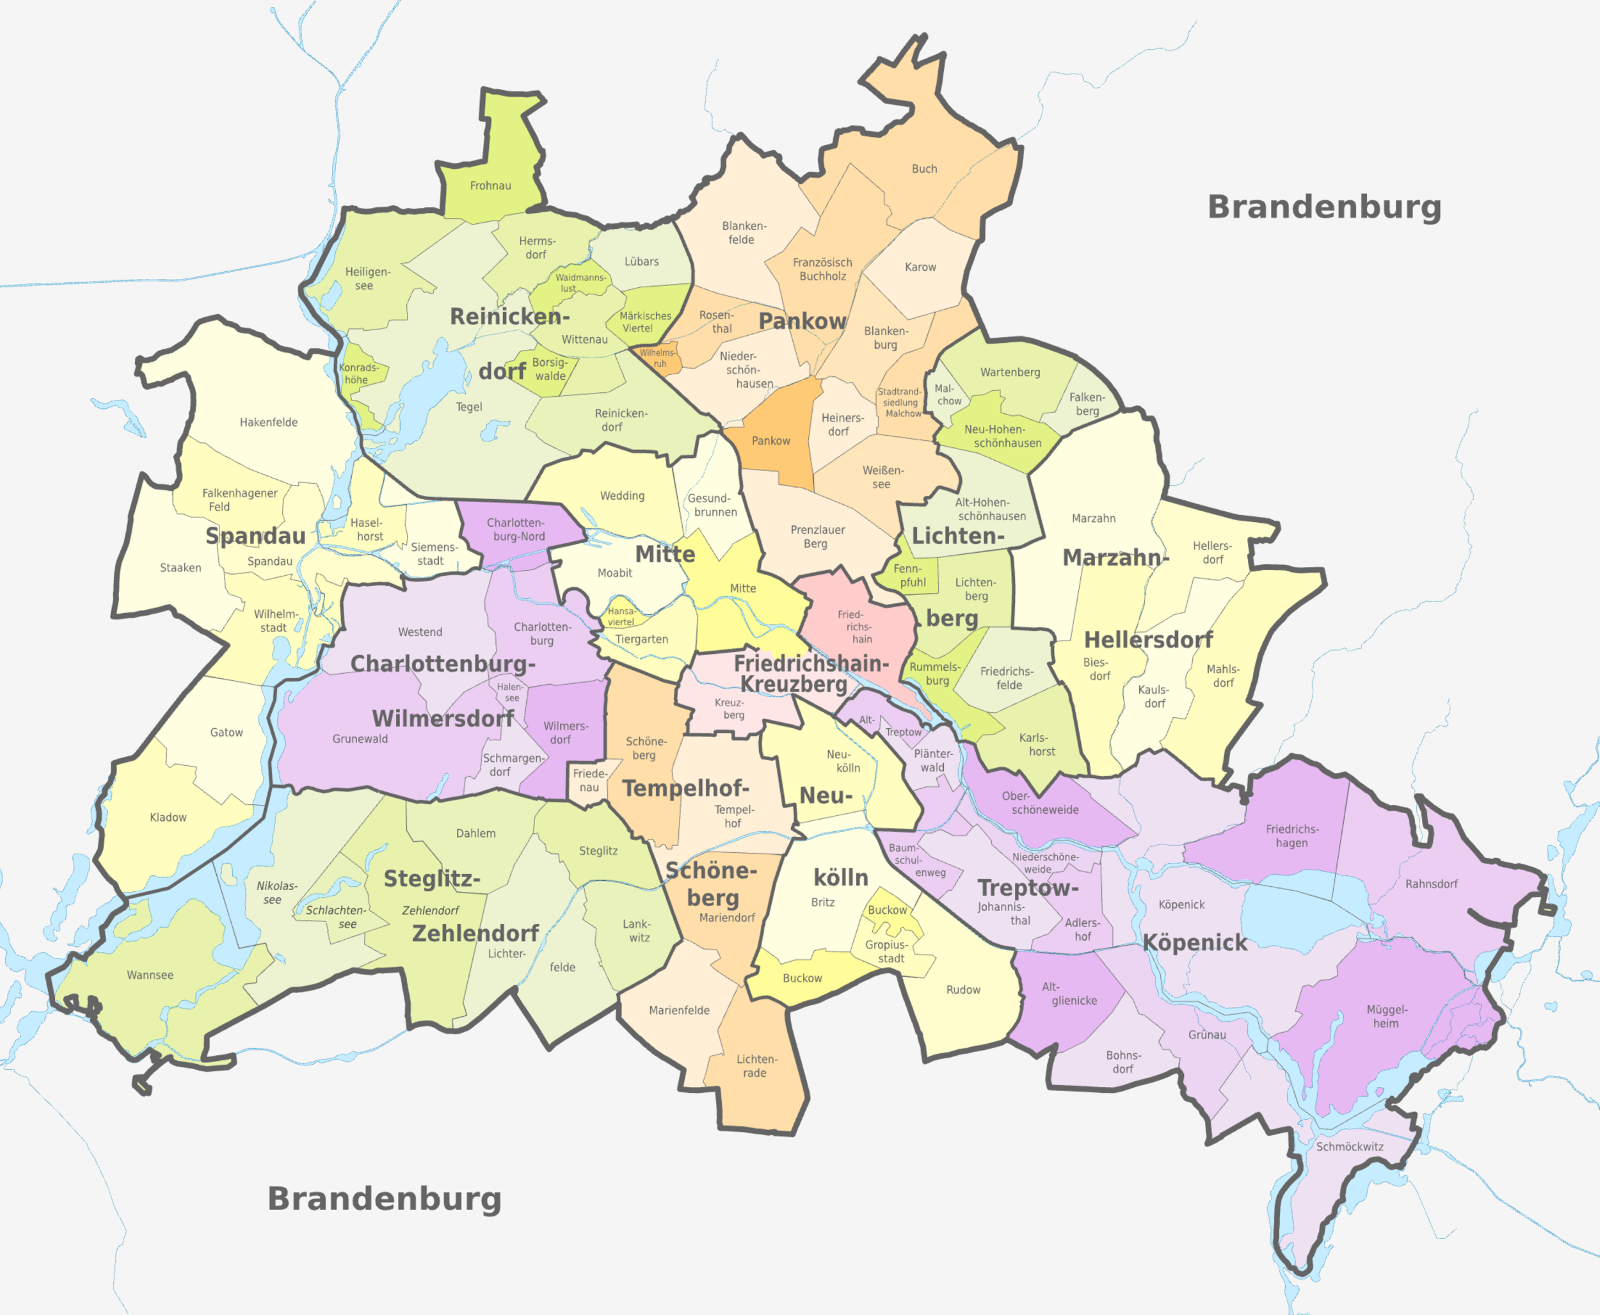
\includegraphics[width=\textwidth]{./figures/intro_rishabh/1_0.png}
%        \caption{}
%        \label{fig:image1}
%    \end{subfigure}
%    \hfill
%    \begin{subfigure}[b]{0.45\textwidth}
%        \centering
%        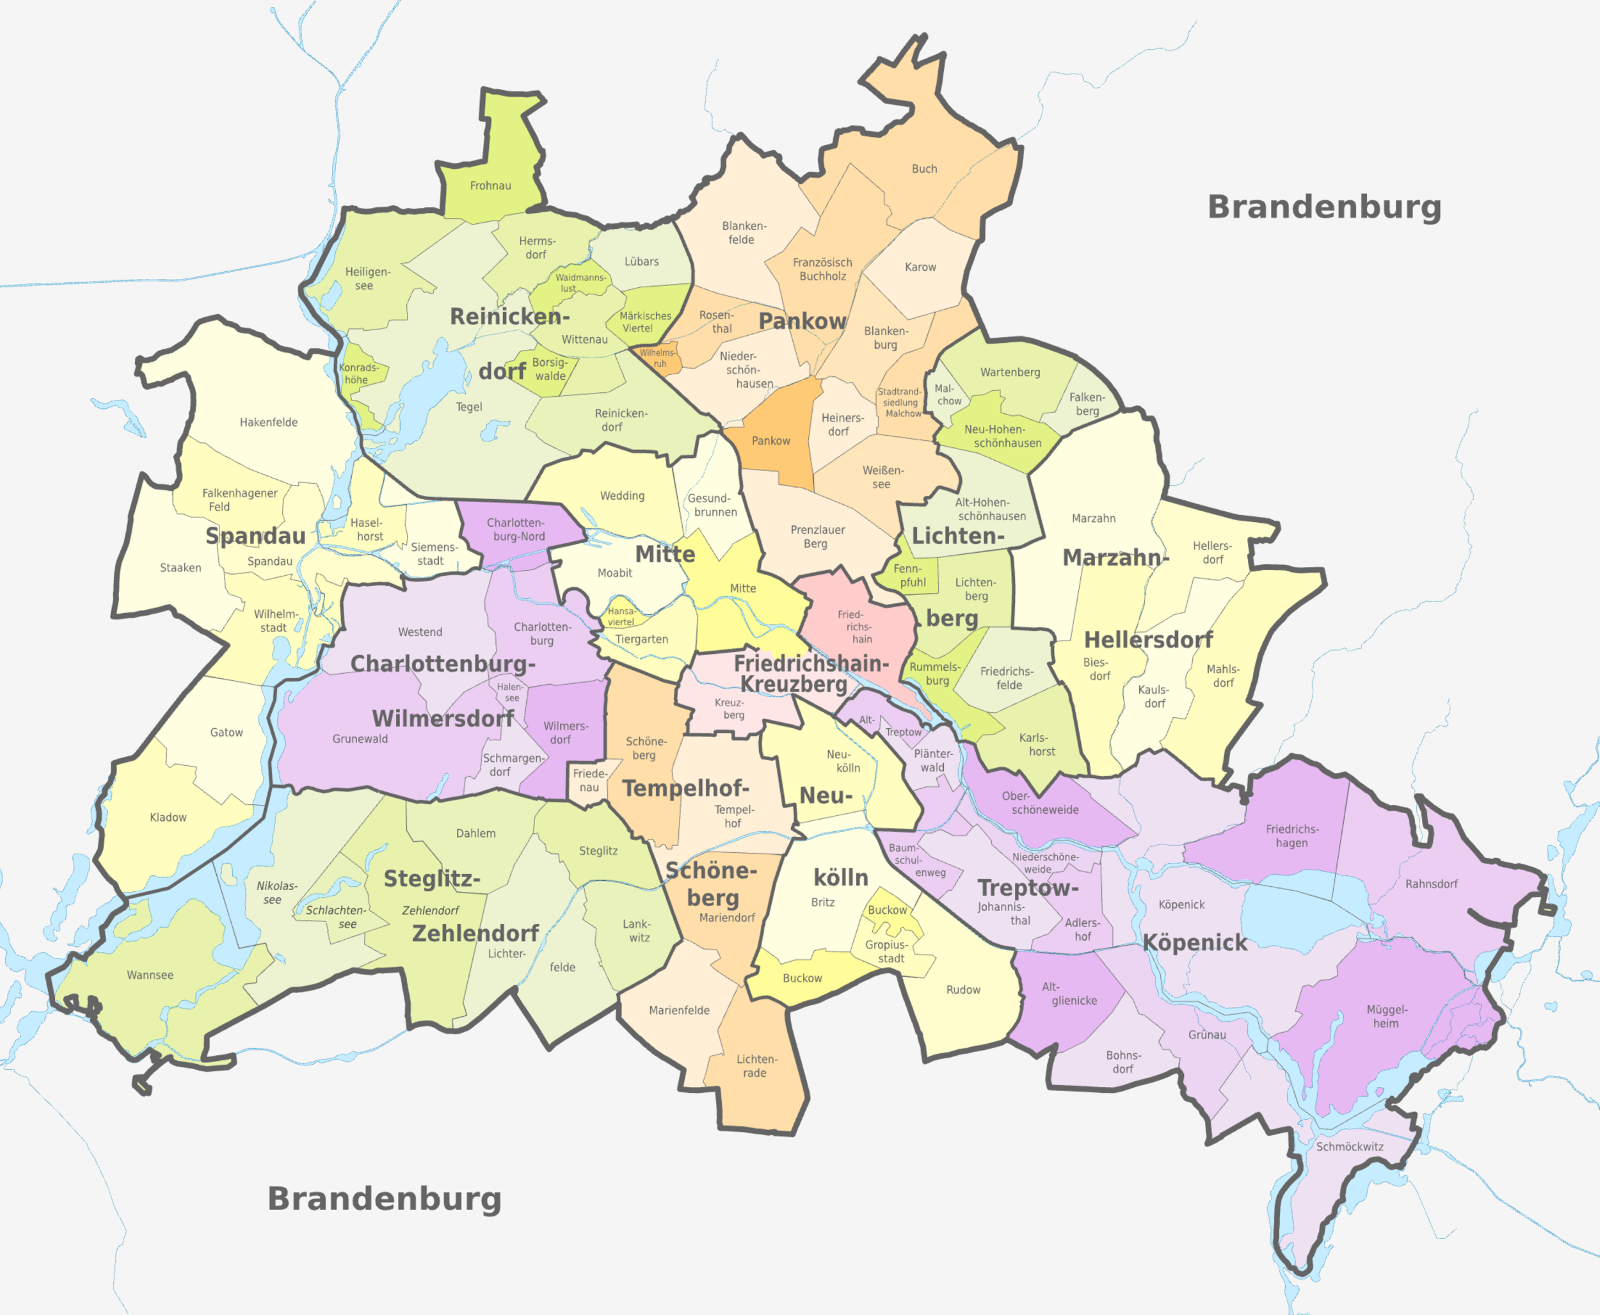
\includegraphics[width=\textwidth]{./figures/intro_rishabh/1_0.png}
%        \caption{}
%        \label{fig:image2}
%    \end{subfigure}
%
%\end{figure}
%\textbf{Crime and Transport Infrastructure Distribution:} Crimes are dispersed throughout Neukölln, with notable clustering in the central and northern regions. Similarly, transport infrastructure locations show higher densities in these areas, leading to a significant overlap. 
%
% \textbf{Density and Proximity:} The high density of transport infrastructure locations in the central and northern parts correlates with the higher frequency of crimes in these regions. This suggests a spatial relationship where areas with more transport infrastructure attract more crime. 
%
% \textbf{Distance Relationship:} The histogram's left-skewed distribution indicates that many crimes occur in close proximity to transport infrastructure locations. A substantial proportion of crimes occur within 200 meters of transport infrastructure locations, supporting the notion that crimes are more frequent near these locations. 
%
% \textbf{Spatial Correlation:} The spatial analysis indicates a notable correlation between crime locations and the presence of transport infrastructure locations. The clustering of crimes near high-density areas with transport infrastructure suggests that these areas might attract more criminal activity due to the gatherings and social interactions associated with transport hubs. 
%
% The analysis reveals a significant correlation between the locations of crimes and transport infrastructure locations in Neukölln. Crimes tend to cluster in regions with a higher density of transport facilities, particularly in the central and northern parts of the area. This spatial relationship suggests that areas with frequent transport activities may attract more crime, possibly due to the increased presence of people frequenting these locations. However, to gain a comprehensive understanding of the factors influencing crime patterns, further analysis incorporating temporal data and additional socio-economic variables is necessary. 
\subsection{Others}
The map shows the distribution of crimes and other infrastructure locations (heatmap) within Neukölln. The categories for other infrastructure include the following: bench, camera surveillance, drinking water, fountain, toilet, tower, waste basket, and water well. 
\begin{figure}[h]
    \centering
    \begin{subfigure}[b]{0.45\textwidth}
        \centering
        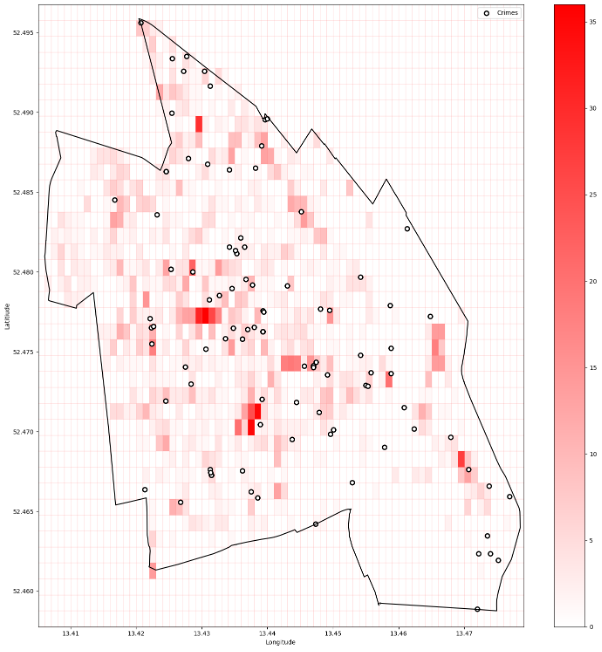
\includegraphics[width=\textwidth]{./figures/Gerard/others.png}
        \caption{}
        \label{fig:image1}
    \end{subfigure}
    \hfill
    \begin{subfigure}[b]{0.45\textwidth}
        \centering
        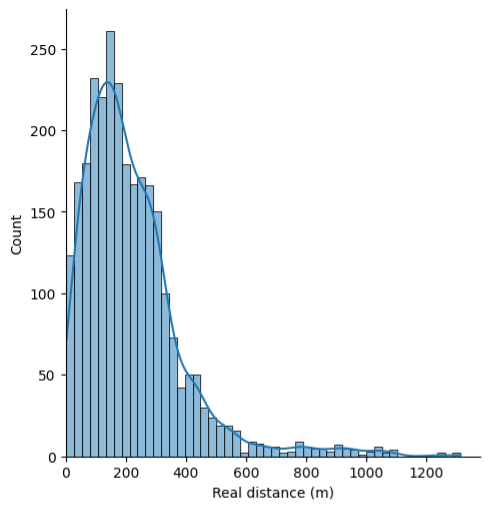
\includegraphics[width=\textwidth]{./figures/Gerard/others_1.png}
        \caption{}
        \label{fig:image2}
    \end{subfigure}

\end{figure}

The histogram shows the minimum distance between each crime and the closest other infrastructure location. 

 \textbf{Crime and Other Infrastructure Distribution:} Crimes are dispersed throughout Neukölln, with notable clustering in the central and northern regions. Similarly, other infrastructure locations show higher densities in these areas, leading to a significant overlap. 

 \textbf{Density and Proximity:} The high density of other infrastructure locations in the central and northern parts correlates with the higher frequency of crimes in these regions. This suggests a spatial relationship where areas with more infrastructure attract more crime. 

 \textbf{Distance Relationship:} The histogram's left-skewed distribution indicates that many crimes occur in close proximity to other infrastructure locations. A substantial proportion of crimes occur within 200 meters of other infrastructure locations, supporting the notion that crimes are more frequent near these locations. 

 \textbf{Spatial Correlation:} The spatial analysis indicates a notable correlation between crime locations and the presence of other infrastructure locations. The clustering of crimes near high-density areas with other infrastructure suggests that these areas might attract more criminal activity due to the gatherings and social interactions associated with these facilities. 

The analysis reveals a significant correlation between the locations of crimes and other infrastructure locations in Neukölln. Crimes tend to cluster in regions with a higher density of infrastructure facilities, particularly in the central and northern parts of the area. This spatial relationship suggests that areas with frequent use of these facilities may attract more crime, possibly due to the increased presence of people frequenting these locations. However, to gain a comprehensive understanding of the factors influencing crime patterns, further analysis incorporating temporal data and additional socio-economic variables is necessary. 